%% The comment character in TeX / LaTeX is the percent character.
%% The following chunk is called the header

\documentclass{article}	% essential first line
\usepackage{times}		% this uses fonts which will look nice in PDF format
\usepackage{graphicx}		% needed for the figures
\usepackage{url}
\usepackage{adjustbox}
\usepackage{amsmath}
\usepackage{listings}
\usepackage{multicol}
\usepackage{color}
\usepackage{multirow}
\usepackage{array}
\usepackage{tabularx}

%% Set the folder where pictures are located
\graphicspath{ {images/} {../poster/images/} }

%% Here I adjust the margins

\oddsidemargin -0.5in%-0.25in		% Left margin is 1in + this value
\textwidth 7.5in		% Right margin is not set explicitly
\topmargin 0in			% Top margin is 1in + this value
\textheight 9in			% Bottom margin is not set explicitly
\columnsep -0.25in %0.25in		% separation between columns

% vplace enviornment
\newenvironment{vplace}[1][1]
  {\par\vspace*{\stretch{#1}}}
  {\vspace*{\stretch{1}}\par}

% set listing settings
\lstset{language=C, 
		numbers=left,
		frame=single,
		tabsize=2,
		breaklines=true,
		commentstyle=\color{red}}

%% Define the fields to be displayed by a \maketitle command
\author{Dee, Timothy\\
    \texttt{timdee@iastate.edu}
    \and
    Long, Justin\\
    \texttt{jlong@iastate.edu}
    \and
    McDonnel, Brandon\\
    \texttt{bmcdonnel@iastate.edu}
}

\title{Remotely Connected Electric Field Generator\\
for Particle Separation in a Fluid \\
\large{Team May1612}}

%%
%% Header now finished
%%

\begin{document}

%\begin{vplace}[0.7]
\thispagestyle{empty}
\maketitle
%\end{vplace}

\newpage
\tableofcontents
\newpage

\begin{multicols}{2}

\abstract{
This document details the design and implementation of a
remotely connected electric field generator.
The goal of this design is to provide an easy interface for
manipulating the output voltage and frequency of a circuit
remotely in order to generate an electric field.
This electric field,
when applied to a fluid over a long period of time
will cause particles in the fluid to separate.
The hardware and software components used to accomplish
the aforementioned goal are described in detail.
}

% Make an argument for why this project is:
% useful
% necessary
% novel
\section{Introduction}
New research has shown that certain particles may be separated from fluids through dielectrophoresis.
This process involves applying an electric field to a fluid.
The field may be manipulated in order to attract or repel certain particles.
The particles the electric field will attract or repel depends on
characteristics of the electric filed which may be controlled
by varying the voltage and frequency of the electronics driving the field.

This technology has many useful applications in health care.
The proposed end use of this equipment is
for separating particles bodily fluids,
such as spinal fluid.
Such medial applications could be useful
in testing or filtering these fluids.

Being capable of separating though the
application of an electric field would represent
an advancement over existing solutions.
It introduces a new method of testing which
could be more precise when compared
to existing technologies.
% TODO

\section{Project Definition}
In our implementation, an electric field is applied 
to two metal plates.
Through varying the voltage and frequency
applied to these plates, 
the properties of the electric field may be changed.

Our job is to construct a system 
containing an electronic circuit capable of providing
the necessary voltages and frequencies required 
to drive a pair of metal plates.
This system must enable the circuit to be controllable 
through the use of a web interface.
In addition, a small form factor must be maintained.

The system must be able to generate up to a 60 V peak-peak sine wave with
user-controlled variable frequency from 10 kHz to 1 MHz. 
% TODO

\subsection{Deliverables}
There are four items which must be constructed for this project:
% TODO list the components which must be constructed

For the analog circuit components,
functionality of the circuit will be tested
using an oscilloscope to verify 
the requirements have been satisfied.
This method can also be used to ensure 
the output signal contains minimal amounts of noise and distortion. 

% TODO if we don't get to the research component of the project,
% we should remove this
The construction of this device is the first phase of the project.
After the completion of this component,
the device will be used 
to experiment with particle separation in various fluid types.
These experiments constitute the remainder of the project.
% TODO add adam's name
For these experiments our advisor at Minetronix, John Pritchard, 
will be the main source of guidance and testable material. 

\subsection{Constraints}
Constraints on this project fall within the size, voltage, and portability domains.

The size requirements of this project are directly related 
to the portability of the final design.
The design requirements specify this system must be easily and quickly
moved around from one workstation to another.
The maximal allowed size is approximately 
the size of a backpack 
with smaller sizes being more desirable
but not explicitly required.
With the electronics currently being used,
these requirements will easily be met.

Another constraint arises from the power supply requirements.
The power supply must deliver at least 60V DC in order to feed the amplifier circuit. 
Due to this, the final design requires a power brick
similar to one which would be used to charge a laptop.
Importantly, this would require the device to be plugged into a wall outlet.
This is not seen as an issue.
Every location this device will operate 
will most likely have other equipment with similar power requirements.

In order to use this system,
there are other items which are required
apart from the device itself. 
The first requirement is a network connection between the device and a computer.
This connection is necessary to be able to interact with the web server hosted on the Raspberry Pi. 
Without a computer to interact with this system there is no practical means of utilizing the device's functionality. 
The next requirement, as mentioned above, is a network connection to the Raspberry Pi. 
The third system requirement is a standard wall outlet
to accommodate the power needs of the system. 

\subsection{System Analysis}
A user will interface with this system though the web interface.
This web interface may be accessed by
typing the IP address of the device into a standard web browser.
The interface will allow the user to choose the values for Voltage and Frequency.
Once these values have been entered,
update scripts on the Raspberry Pi
will set the voltage and frequency output of the circuit
according to the values entered.

%\section{Block Diagram}
\begin{figure*}[!hbt]
\begin{center}
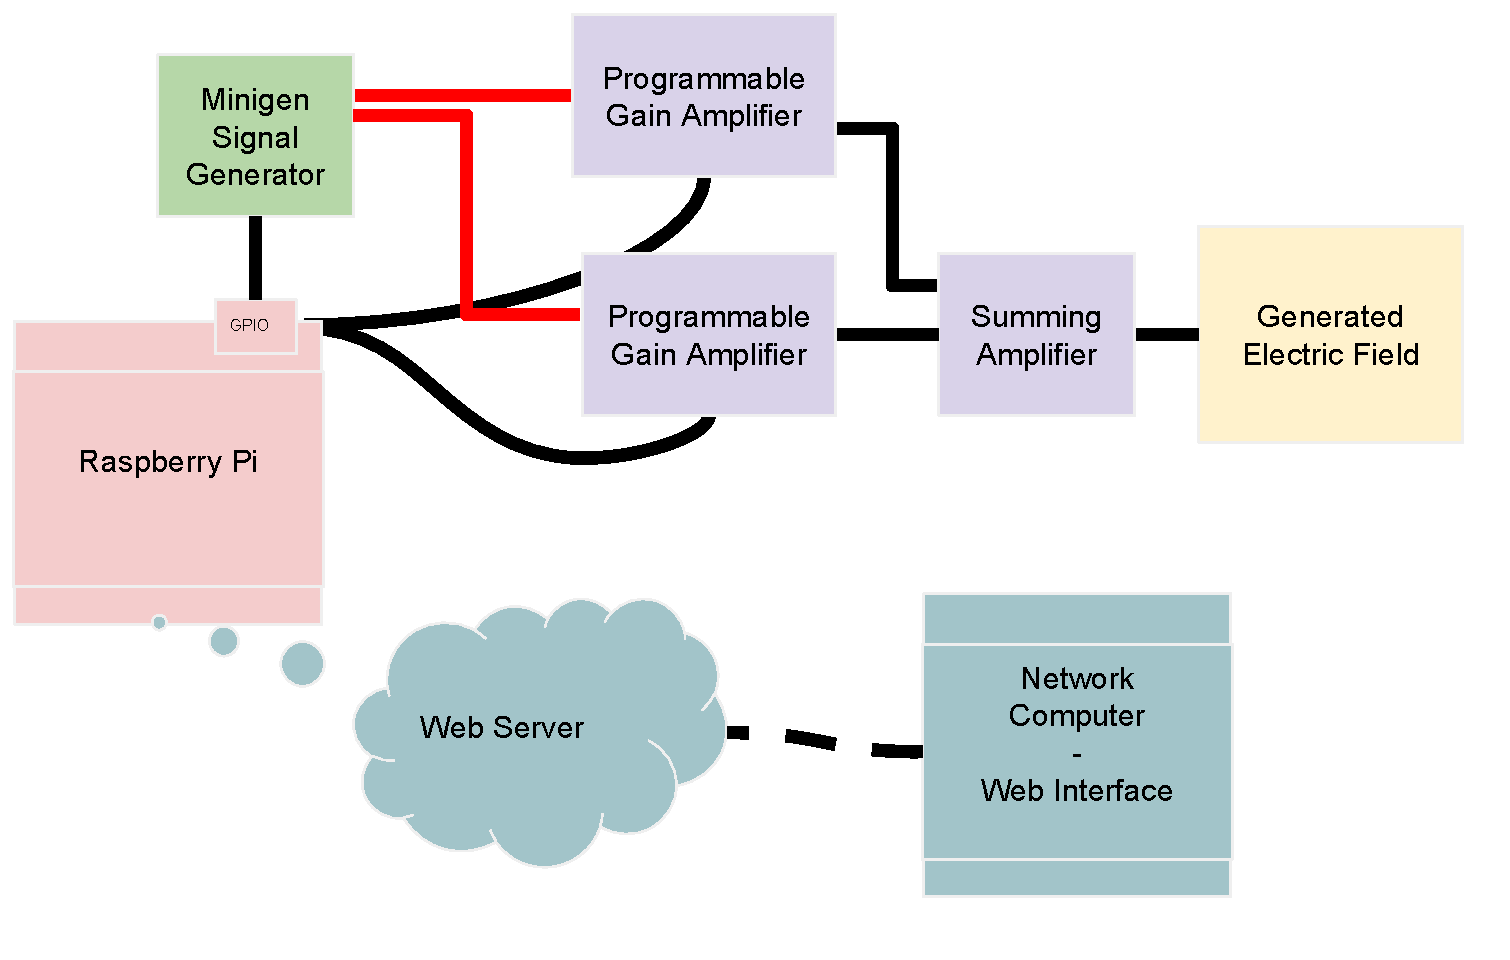
\includegraphics[width=1.0\textwidth,keepaspectratio]{block_diagram.png}
\end{center}
\caption{Block Diagram provides an overview of the system components.}
\end{figure*}

\section{Functional Decomposition}
This system has four fundamental functional blocks.
These include the 
Web Interface, 
Raspberry Pi, 
Minigen Signal Generator, and
Amplifier Circuit.
The project will be described in terms of 
these components and
their interactions.

\subsection{Raspberry Pi}
The Raspberry Pi will act as the bridge between the user and the circuit.
The Raspberry Pi will host a web server allowing the user to interact with the system.
Based on the results of this user interaction, 
the Raspberry Pi will update the state of the GPIO pins.
The GPIO pins connect to a circuit causing the output to change based on their state. 

In addition to hosting the web server the Raspberry pi is used to
communicate with the 
Minigen Signal Generator and 
amplifier circuit.
This communication is accomplished via 
the Raspberry Pi's SPI interface and
GPIO pins respectively.

%TODO

%TODO insert Raspberry Pi connection diagram
\begin{center}
\includegraphics[width=0.45\textwidth,keepaspectratio]{rpi_real.png}
\end{center}

\subsection{Minigen}
The Minigen Function Generator device controls the frequency output by the circuit.
Varying the frequency is accomplished 
by writing to registers present on the Minigen.
This communication is completed over SPI between
the Raspberry Pi and the Minigen.
The frequency produced is a function of
the values contained in the Minigen's frequency registers.

The Minigen outputs a waveform 
from -0.5V to 0.5V. 
This waveform may be a triangle, square, or sine wave.
The voltage output by the Minigen is not variable.
Given that the design specification requires a variable voltage,
the voltage needs to be adjusted separately.
Accordingly, the output of the Minigen 
is supplied to the input of the amplifier circuit.

The Minigen is controlled by setting five registers,
two registers for frequency, 
two for phase shift and 
one as a control. 
There exists no need for phase shifting
to meet the design requirements, 
however the frequency and control registers
are needed. 
By having two frequency registers,
data can be sent to one register while it is not in use,
followed by a write to the control register to use this register.
This allows for a nicer gradient, 
because the frequency will not change until the entire frequency register is written. 
The control register also allows for changing between sine, square and triangle waveforms.
In the event that the frequency needs to be finely adjusted,
this system utilizes the functionality of the control register
to modify the way in which writes to the frequency registers are received.
The way writes are received by the frequency registers 
can be varied between two modes.
In one mode,
two consecutive 14-bit writes to a frequency register are used.
In the other mode,
one write to the lower 14-bits of the 28-bit frequency register is used.
This functionality affords the ability to accurately dial in small changes to the register values quickly.

\begin{center}
\includegraphics[width=0.45\textwidth,keepaspectratio]{minigen_real.png}
\end{center}

Until this point,
several functional benefits of the Minigen Signal Generator have been discussed.
An additional benefit which 
increases the practicality of this solution is the Minigen's small form factor.
The small chip size 
allows the Minigen to fit easily into a small case 
with the Raspberry Pi.
This is consistent with the system's requisite small footprint.

\subsection{Amplifier Circuit}
As mentioned in the previous section,
the output of the Minigen Function Generator
is applied to the amplifier circuit as input.
The amplifier also receives input from 
the GPIO pins of the Raspberry Pi.
These GPIO pins act as switches which help to control the output voltage.
Based on these inputs 
the amplifier circuit manages the overall 
voltage and frequency output.

The project requirements state that the system must 
generate signals which range from $1V_{pp}$ to $60V_{pp}$. 
To accomplish this,
various circuit components were used to accomplish the amplification.
The overall scheme is to split the output voltages into
three different ranges.
One component is used to adjust the voltage within each of the ranges while
other comp are used to change the range the voltage adjuster is acting within.

A schematic illustrating the amplifier circuit as a whole is 
%TODO

\begin{figure*}[!hbt]
\begin{center}
\includegraphics[width=0.8\textwidth,keepaspectratio]{circuit_diagram.pdf}
\end{center}
\caption{Amplifier circuit design to vary voltage 
    within range $1V_{pp}$ to $60V_{pp}$. }
\end{figure*}

\subsubsection{Summing Amplifier}
The summing amplifier is the last component
in the amplifier circuit.
The overall voltage range which needs to be produced is divided into three segments.
Each of these segments have their output connected as
input to the summing amplifier.
One of the segments utilizes a programmable gain amplifier(PGA)
to vary the voltage within one third of the range.
While the relays are used to increase the voltage by one third of the overall voltage range when they are turned on.

The advantage of this design is that
it allows for three times the number of voltage steps
allowed for by a single PGA.
This could also be accomplished by using multiple PGA's.
Utilizing the relays in increase the voltage instead of additional PGA's
allows for reduced software and hardware complexity.

\subsubsection{Programmable Gain Amplifier(PGA)}
There are three $20V_{pp}$ voltage ranges.
Which range being acted in is chosen by the relay circuits.
Within a given range,
however,
a PGA is used to control the voltage output.
In our implementation,
a PGA has control over a $20V_{pp}$ range.
The PGA has 8 steps within this range.
This Device is controlled by 
the SPI interface on the Raspberry Pi.

%TODO

%TODO insert a diagram of the amplifier circuit
%\begin{center}
%\includegraphics[width=0.45\textwidth,keepaspectratio]{amplifier_circuit.png}
%\end{center}

\section{Software Components}
The web interface displayed by
the web server hosted on the Raspberry Pi
is the user's window into the system.
Through this interface,
the user can seamlessly control various
components of the system cause 
the desired voltage and frequency 
to be produced.
Previously covered are
the hardware components used to accomplish this.
This section describes the software counterparts
used to control the hardware.

\subsection{Web Interface}
The web interface is hosted on the Raspberry Pi using an Apache web server.
This web server displays an interface which allows the user to
set a voltage and frequency output by the system. 
The interface is simple and interactive,
implemented using cgi-scripts on the Apache web server.

Our implementation provides several functionalities.
Among these are
the ability to set:
voltage and frequency,
sine or triangle or square waveforms,
and the ability to set a voltage and frequency for an amount of time.
The table displayed
in the figure below
provides the ability to set voltage and frequency for the number
of minutes specified.
The "Go" button will cause the first
voltage and frequency to be set for the corresponding amount of time.
After the time has expired,
the next voltage and frequency will be set for the corresponding amount of time.
This process continues until the table entries are completed or
the user presses the "Stop" button.

\begin{center}
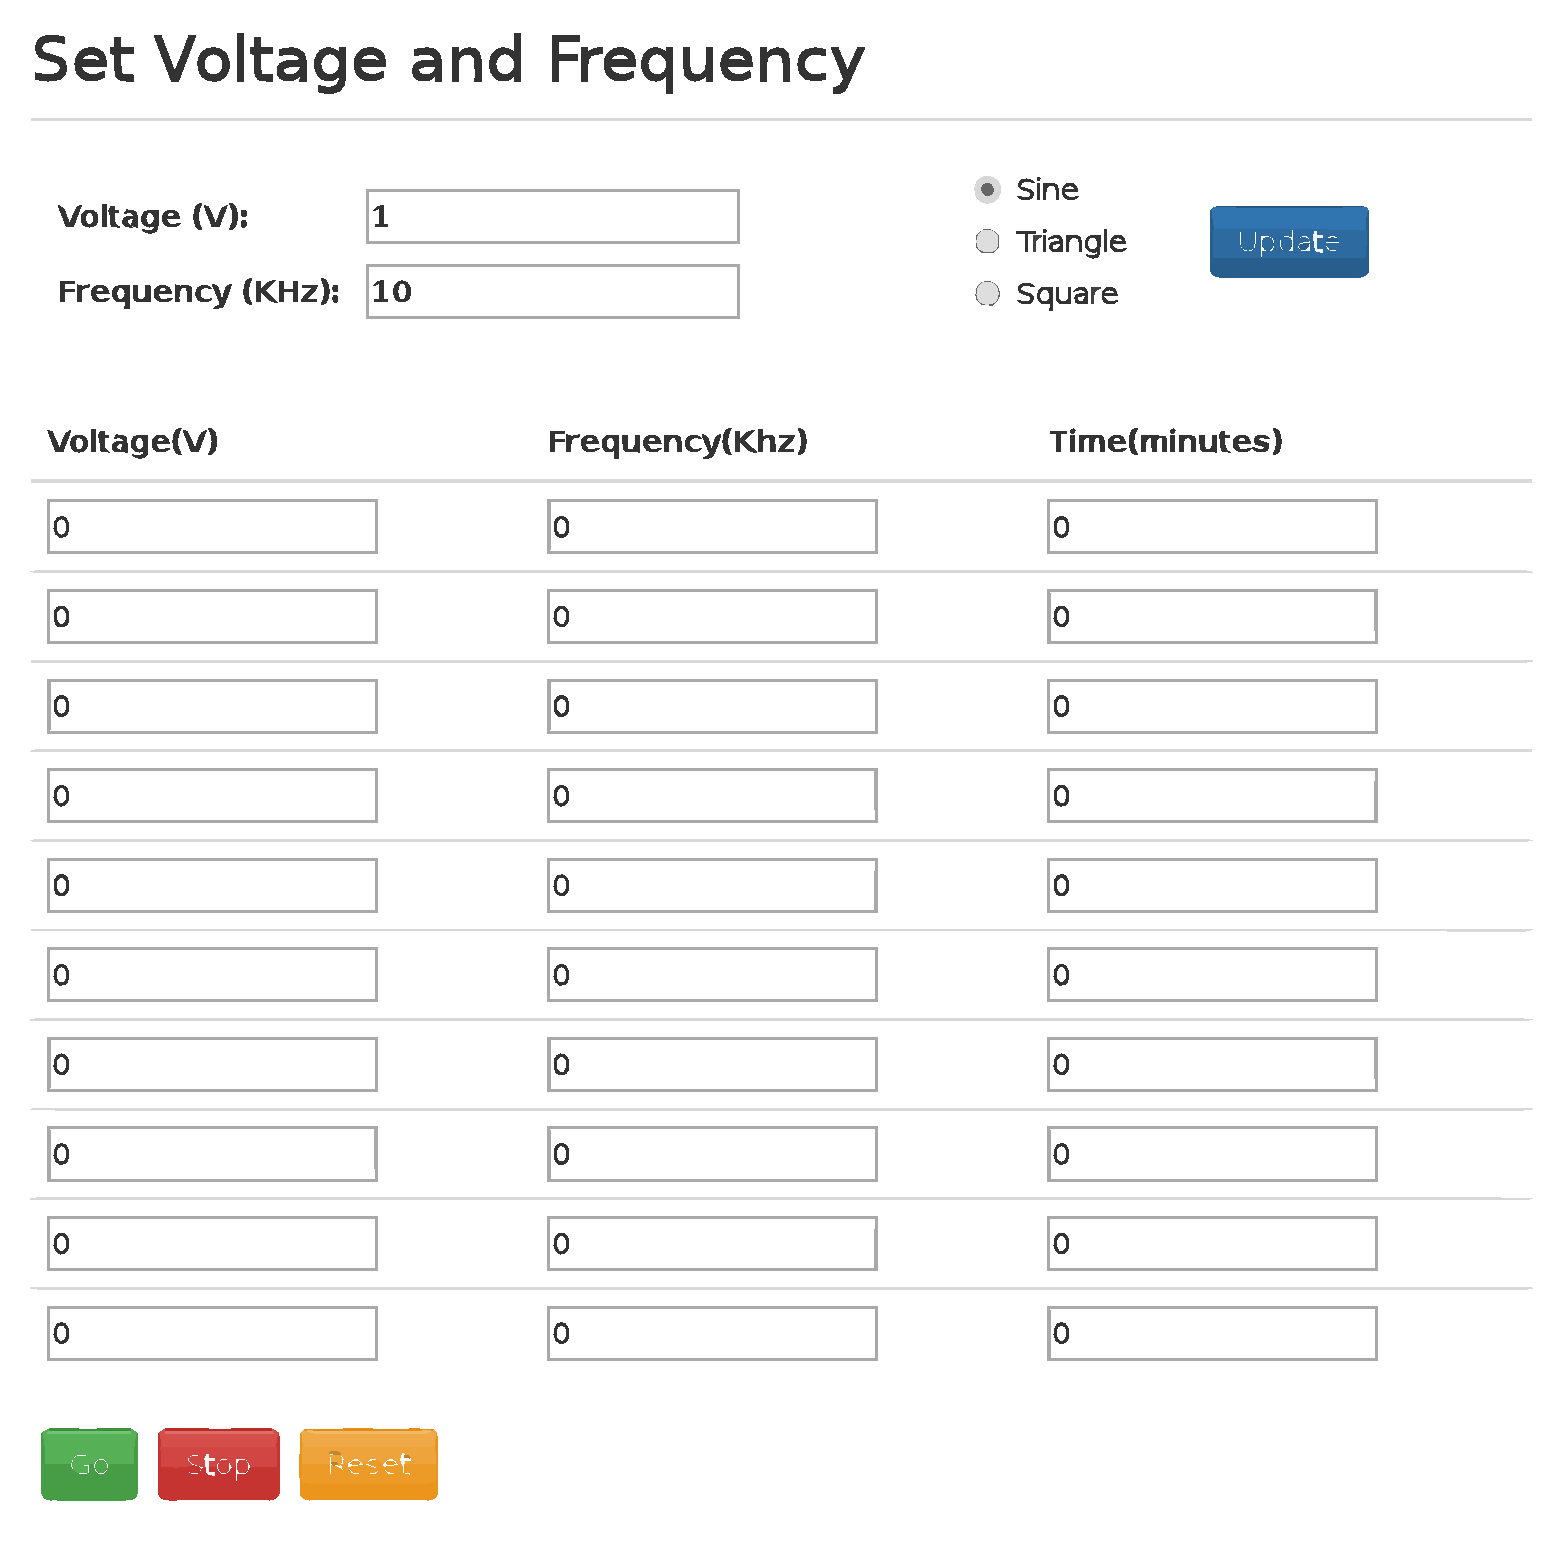
\includegraphics[width=0.45\textwidth,keepaspectratio]{web_interface.pdf}
\end{center}

\subsection{Web Server}
The primary function of the web server is to communicate with the Raspberry Pi.
This is the primary method of control afforded 
to the user by the system. 
The web pages displayed by the server
have the ability to control the voltage and frequency output by the circuit.

Displaying this interface is accomplished by 
running an Apache web server on the Raspberry Pi. 
When the user clicks update, the server could executes 
a cgi-script performing the update functionality.

% code layout diagram
%\begin{figure}[!hbt]
\begin{center}
\includegraphics[width=0.45\textwidth,keepaspectratio]{script_layout.png}
\end{center}
%\caption{Script layout according to work delegation.}
%\label{fig_script_layout}
%\end{figure}

\subsection{Modifying Frequency}
The frequency output by the circuit is controlled 
by the Minigen Function Generator.
Thus the software components used to 
modify the output frequency
are in essence
a method of communication with the Minigen device.

The process begins when the user 
enters a new frequency value into the web interface
and clicks the "update" button.
The \textit{update.py} script parses 
the parameters contained in the URL
resulting from the user's update request.
These parameters are than
passed on to \textit{update\_voltage\_frequency.py}
which determines the appropriate update procedure 
with which to call \textit{minigen.py}.

%TODO explain how minigen.py works in detail

\subsection{Controlling Voltage}

\subsubsection{Programmable Gain Amplifier(PGA)}
%TODO explain how we choose the value to set the pga
%TODO explain how we modify the value of the pga


\section{Cost Considerations}
The monetary cost of this project is fairly low. 
The precise costs of components in the future are unknown, but
a table 
of current prices has been provided
along with the necessary quantity of each component.
The projected cost of op-amps and other electronic components is minimal. 
The largest expenditure of the project is
the purchase of the 
Raspberry Pi 2 and 
Minigen Function Generator. 
The Raspberry Pi 2 package is currently priced at \$99.95 and
the Minigen cost at \$29.95.
Thinking conservatively the cost of the major hardware will be \$129.90. 
In addition, the cost of 
a resistor kit, 
a capacitor kit, and 
a handful of op-amps 
must be included.

%The Minigen Function Generator may be acquired from 
%\textit{http://www.sparkfun.com}.
%This website also provides 
%a resistor kit for \$7.95 
%which includes all necessary resistors. 
%From this same website,
%individual capacitors may be purchased
%at a rate of \$0.25 per capacitor.
%Operational amplifiers may also be purchased at
%a rate of \$0.95 per amplifier.
%Given this,
%the total cost is approximated at \$152.35. 
%This is far below the maximum allotted funds of \$1,000
%specified in the project description.

%TODO table of costs
\begin{center}
    \begin{tabularx}{0.4\textwidth}{|X|X|X|X|}
        \hline

        \textbf{Item} &
        \textbf{Part Number} &
        \textbf{Quantity} &
        \textbf{Price(\$)} \\
        \hline

        \textbf{Raspberry Pi 3 Kit} &
        \textbf{-} &
        \textbf{1} &
        \textbf{49.99} \\
        \hline

        \textbf{Minigen Function Generator} &
        \textbf{AD9837} &
        \textbf{1} &
        \textbf{29.95} \\
        \hline

        \textbf{Resistor Pack} &
        \textbf{-} &
        \textbf{1} &
        \textbf{7.95} \\
        \hline

        \textbf{Capacitor Pack} &
        \textbf{-} &
        \textbf{1} &
        \textbf{7.95} \\
        \hline

        \textbf{Op Amps} &
        \textbf{-} &
        \textbf{8} &
        \textbf{9.50} \\
        \hline

        \textbf{Total} &
        \textbf{-} &
        \textbf{-} &
        \textbf{102.35} \\

        \hline
    \end{tabularx}
\end{center}

\section{Testing}
In order to discuss testing in a more clear way
it is useful to define a number of steps
in the testing process.
Each of these steps can than be developed for
each of the various components to the project.
%
The flow of the testing process
involved an iterative process of:
\begin{enumerate}
\item Theorize a design
\item Acquire necessary components
    \begin{itemize}
    \item knowledge
    \item hardware components
    \end{itemize}
\item Implement design
\item Understand problems
\item Return to step 1
\end{enumerate}
%
It is important to recognize that many
of these steps may be different for different components.
A program written to be run by the web server
will inevitably have different testing requirements from
a new integrated circuit component.

% elaborate on each step of the process 
% describe how each component is affected at each step
% discuss the goal of each phase
\subsection{Testing Process}
Each phase of the testing process poses unique challenges.
Here are presented some of those challenges and
how each phase related to specific aspects of this project.
Importantly, the time it takes to complete a 
testing cycle varies drastically.
Hardware components, for instance, take far longer to test
as they must be constructed on a breadboard in order that 
measurements may be taken with lab equipment.
%
The length of the testing cycle is 
directly proportional to the extent to
which a component may be tested.
%
For objects with long testing cycles,
much more time is spent in the 
theorizing a design phase compared to
objects with shorter testing cycles.

\subsubsection{Theorize a design}
In this phase of development,
the goal is to determine:
\begin{itemize}
\item A design which \emph{should} work
\item What knowledge is needed to complete an implementation
\item What physical components will be necessary
\end{itemize}

Often times it is wise to determine the above for
multiple potential solutions.
The time necessary to implement each solution
can then be estimated and weighed against
the potential for success with such a design.

Which design is chosen for implementation is
some combination of the estimated time and
potential for success.
The decision to abandon a design is often
due to a change in one of these factors.
This change can occur either
in the current design or
in one of the alternative designs.
An example which might motivate abandonment of a 
particular solution might be
the finding that a certain hardware component
contained in the current design is incapable of 
working at a high enough frequency to
produce the overall output.

% cover hardware and software components and differances in this phase between them
While the theory of testing hardware and software is similar,
in practice these activities can be very different.
In this project, however,
they became somewhat similar 
due to the fact that program code is written in order to 
interact with hardware components.
In both cases,
the physical output of either GPIO pins on the Raspberry Pi
or output of a circuit component must be view on
an oscilloscope.

\subsubsection{Acquire necessary components}
The goal of this phase is self-explanatory.
The necessary components must be acquired.
While the goal may be clear and simple;
it may not be easy.
The term acquisition may refer to  physical hardware,
but it also refers to the knowledge necessary to implement
a given system.
Every potential implementation has a knowledge component.
Even if the knowledge is already known by the group as a whole,
it may be useful to consolidate the information.

Fundamentally this process tries to answer the question,
"What do I need to know in order to create x result".
Where x is the goal of the component as a whole, or
x is a subgoal which is thought to contribute to 
the overall goal of the component.
This phase of testing
sets the theorized design against existing knowledge.
Often times it is necessary to return to the 
theorizing phase and reconstitute the design
given new information which has been acquired.

% illustrate the differences between acquiring hardware and software components
Acquiring components phase has analogs in both hardware and software domains.
In the software domain,
acquiring components consists of
software packages, such a Apache 2, or
knowledge assets necessary to complete a program.
In the case of this project,
we needed to learn how to use and configure apache,
write Python code on the Raspberry Pi,
use py-spi in order to communicate with the Minigen, and
use GPIO library on Raspberry Pi to communicate with the PGA components.

Compare this to the hardware domain where
the acquisition of components is fairly straightforward.
Components are necessary to be purchased.
This process takes much longer when compared
to downloading a software package.
Thus, it is useful, wise, and resource efficient to
spend much more time in the theorizing a design phase.
Having an increased degree of certainty that 
a given component will preform as expected
alleviates the time and money required to determine 
that a component will not work empirically.
This certainty can be developed though simulations, or
developing a mathematical description of the output of a design.

\subsubsection{Implement design}
Of all the phases, 
this phase constitutes the largest investment.
The majority of time spent on the project is
used to implement a design.
The goal of this phase is both obvious
and complex.

An increased degree of efficiency may be achieved by
constructing a minimal working example(MWE).
The benefit in doing this is twofold.
First, a MWE is often easier to construct compared to
a version which is constructed into the other
components of the project.
Second, because constructing a MWE requires that
this sample implementation not be integrated into
the rest of the project,
issues which arise from the interplay between devices are not present.
This helps to isolate issues which are a product
of the specific aspect of the project which is being implemented.

% discuss differences between hardware and software implementations
Implementing designs in hardware is significantly different compared to software.
Hardware designs must be constructed with physical components on a breadboard.
These components must be connected and measured with lab equipment
in order to determine if the components are having the correct output.
All the steps in this process take time.
Other issues also exist due to the physical nature of 
hardware components.
A component might be partially burned out and providing output
which is not correct, but still proving output.
The difficulty with this is that the component appears
the same as it would if it were connected incorrectly.
For these reasons,
the Implementing a design phase 
consumes many more resources in the time and economic
domains compared to software implementations.

\subsubsection{Understand problems}
After implementation of the design is complete,
it must be determined whether or not the device functions
as expected.
Often times this means looking at the input and
output waveforms on an oscilloscope for hardware or
observing the change in state of the GPIO pins for
testing software.
Once a problem has been identified,
the source of the problem must be located.

To clarify the above point, consider 
an example of a problem which might be observed is
a difference in amplitude of the output waveform
compared to what was expected.
The problem might be any component which is
connected to the measured point.
This includes components which are connected
via other components.

Often times to identify the source of an issue,
it is necessary to understand what should be
the input and output of all components in the circuit.
Testing the inputs and outputs of each component in turn
moving away from the originally observed wrong output can
help to find where the origin of the problem occurred.
Perhaps the component which gives input the component
previous the the component with the observed problem
is connected incorrectly.
This could cause the output of all future components to become incorrect.

A similarity between debugging code and
finding issues in hardware implementations is
the effect of mistakes.
The way a mistake propagates though a
program is similar to the way mistakes
propagate though hardware implementations.
All events after the first error are
often a result of the first error.
There fore these events are also in error.
Often times a good debugging strategy is
to approach solving the first error.
The benefit in doing this is that future errors
might be solved indirectly.

\subsubsection{Return to step 1}
Many times it is found that designs would not work
and thus this process is reset to the beginning.
This step can be disheartening, but
it is wholly necessary.
Emotions of anguish may cloud a person's judgment
causing them to stick with a particular implementation
for far longer than what is necessary to determine 
better solutions exist.
Developing a control over these emotions
yields decisions which reduce the time
taken to complete a project and
often produce better results.

Much wisdom is needed to be able to objectively 
evaluate one's current situation and determine 
whether it is advisable to
continue down the current path or whether
The new information gathered in the "understanding problems" phase
warrants the construction of a new design 
or significant portion of design.
Often times this can be reduced to answering the following question honestly,
"Given what is now known,
is it wise to invest in the current course of action, or
is there something else which might have an improved probability of success"

% discuss the difficulties with this with respect to hardware components
In software,
returning to theorizing a consumes far fewer resources compared
to redesigning a hardware implementation.
In software,
new packages may be downloaded nearly instantaneously.
Compare this with hardware where new components must
be chosen, bought, and shipped.
The need to redesign can be expensive and time consuming, but
often times it is wise to do if the current design is not working as expected
to such an extent that another design would be a smarter investment.

\subsection{Testing Results}
Testing occurred in an iterative process
as described above throughout the semester.
Each time a new design would be reached,
the steps above were used to uncover what
the issues were, 
how to solve them, and
whether it was wise to solve them at all.
The alternative to solving current issues is
establishing a new design.

A typical testing environment includes:
\begin{itemize}
\item Oscilloscope
\item Raspberry Pi
  \begin{itemize}
  \item Connected for monitor for web interface access
  \item Connected to circuit to control Minigen, PGA's
  \end{itemize}
\item Multiple breadboards
  \begin{itemize}
  \item Minigen Function Generator
  \item PGA's
  \item Summing amplifier
  \end{itemize}
\end{itemize}

%TODO explain testing results for each of the components

\subsection{Known Issues}
Below are some of the issues found
through the course of our testing
which have not been resolved.
These issues are fairly minor compared
to the overall functionality.

The current solution has some noteworthy issues
which need to be addressed.
Issues are defined as unintended issues of unknown origin.
Possible reasons for each of the issues are discussed as
well as the accommodations made in this implementation to lessen their impact.
Potential solutions are also mentioned.

\subsubsection{B23}
In the current prototype,
there is an ongoing issue with the Minigen Function Generator.
This device works as expected in most cases.
The exception occurs when bit 23 of either frequency register
is set high.
This case will cause the Minigen device to produce a $4Mhz$ sine wave.
There is potential that the specific Minigen device used 
is responsible for this bug.
Further testing is required.

The solution currently implemented is
to detect conditions which will cause the error
and avert these situations problematically.
Whenever bit 23 is set to high in a frequency register write,
the current implementation sets bit 23 to low
and sets all less significant bits to high.

%\subsection{other?}
%TODO

% compare what has been accomplished to the project description
% note the dependencies between them
% detail each difference and highlight why it happened
% conclude with the final state of the project
\section{Concluding Remarks}

%TODO

% go to next page
\pagebreak
\appendix

\section{Operation Manual}
\subsection{Setup}
This section details the materials needed and
how to set them up.
This section assumes you have nothing
other than the
circuit to connect to the Raspberry Pi and
the controlling code which needs to be placed on
the Raspberry Pi.

Setup includes all necessary information
for the Raspberry Pi configuration.
Such information is provided
for the purpose of understanding 
how the system has been established
in hopes that it might be easier to modify or
change in the future.

\textbf{Steps:}
\begin{enumerate}
\item Purchase a Raspberry Pi
    \begin{enumerate}
    \item micro SD card
    \item micro USB power cord
    \item (optional) USB wifi adapter
    \item (optional) Ethernet cable
    \end{enumerate}
\item Install Rasbian Linux Operating System on Raspberry Pi
\item Place circuit controlling software on the Raspberry Pi
\item Install software packages on Raspberry Pi
    \begin{enumerate}
    \item Apache 2 Web Server
    \item TODO python package
    \item TODO python spi package
    \item TODO gpio package
    \end{enumerate}
\item Modify configuration files on the Raspberry Pi
\end{enumerate}

% explain each of the steps
\subsubsection{Purchase a Raspberry Pi}

%TODO 

\subsubsection{Install Rasbian Linux Operating System on Raspberry Pi}
%TODO 

\subsubsection{Place circuit controlling software on the Raspberry Pi}
%TODO 

\subsubsection{Install software packages on Raspberry Pi}
%TODO 

\subsubsection{Modify configuration files on the Raspberry Pi}
%TODO 

\subsection{Demo}
This section details the process
by which a device which has already
been setup may be showcased.
An example use of the system might be as follows.
Connect the output of the circuit to the pair
of capacitive plates which will drive 
the dielectrophoresis experiment.
Once connected,
Connect to the raspberry pi over
the local area network from
any computer on the network and
use the interface to modify the
voltage and frequency output of the circuit.

\textbf{Steps:}
\begin{enumerate}
\item{Power on the Raspberry Pi}
\item{Connect the Raspberry Pi to the network}
\item{The output of the circuit should connect to capacitive plates used for dielectrophoresis}
\item{Acquire the IP address of the Raspberry Pi}
\item{Enter the IP address in the navigation bar of a web browser}
\item{Input the desired voltage and frequency values and click update}
\item{The output of the circuit can be seen to change to the desired values}
\end{enumerate}

% discuss each step
% pictues of each step
\subsubsection{Power on the Raspberry Pi}
In order to power on the Raspberry Pi,
It must be plugged into a wall output.
The power adapter for this device is
the same as any micro USB smart phone adapter.
Once plugged in,
The Raspberry Pi will power up automatically.

Below is pictured the process of
powering on the Raspberry Pi.
%TODO
\begin{center}
\includegraphics[width=0.45\textwidth,keepaspectratio]{power_on_pi.png}
\end{center}

\subsubsection{Connect the Raspberry Pi to the network}
Connecting the Raspberry Pi to the network may
be done in a couple of way:
through the Ethernet port on the Raspberry Pi, or
through a wireless network adapter connected to
one of the Raspberry Pi's USB ports.
Either method of connection will allow
any computer on the local network to 
connect to the web server running on the Raspberry Pi.

\subsubsection{The output of the circuit should connect to capacitive plates used for dielectrophoresis}
Ensure all of the outputs to the circuit are connected properly.
Preforming this step incorrectly can cause damage to the equipment.

\subsubsection{Acquire the IP address of the Raspberry Pi}
Finding the Raspberry pi on the network can be somewhat tricky.
The Raspberry Pi has a display output on board.
If access to this display is available,
a keyboard may be connected to the pi in order to
interact with it.

To acquire the IP address of the Raspberry Pi,
login and run the 'hostname' command with arguments '-i'.
This command is depicted below.
\begin{lstlisting}
# username: pi
# password: pi
# hostname -i
\end{lstlisting}
The output of this command will the the IP address of
the Raspberry Pi on the network.

There are other ways to acquire the IP address
which involve scanning the network from
another computer on the network.
Another way would be to configure a static IP address
for the Raspberry Pi.

Configuring a static IP can be done in a few ways.
One way to accomplish this is
to modify the router setup to assign the Raspberry PI a specific IP.
Another method is to configure the PI to request a specific IP address.

\subsubsection{Enter the IP address in the navigation bar of a web browser}
On any computer connected to the same network as the Raspberry Pi,
open a web browser.
In the navigation bar of this browser,
enter the IP address retrieved from the 'hostname' utility.

%TODO
\begin{center}
\includegraphics[width=0.45\textwidth,keepaspectratio]{ip_in_navigation_bar.png}
\end{center}

\subsubsection{Input the desired voltage and frequency values and click update}
The web interface contains fields to input the desired frequency and voltage values.
Enter these values and click the 'update' button.
Doing so will cause scripts to Run on the Raspberry Pi that
set the values of the GPIO pins in such a way that the output is produced
by the circuit.
There is also a Radio Button group which will allow the 
output waveform to be modified among triangle, square, and sine.

%TODO
\begin{center}
\includegraphics[width=0.45\textwidth,keepaspectratio]{web_interface_updating_values.png}
\end{center}

\subsubsection{The output of the circuit can be seen to change to the desired values}
After the 'update' button is pressed,
the output of the circuit will be modified
to the closest possible values.
The voltage and frequency resolution are limited,
thus the output may not be exactly the value entered.

After update is pressed,
the web interface will be re-displayed.
This will allow the modification of voltage and frequency again.

\newpage
\section{Initial Designs}
This section covers the designs that have been tried
throughout the course of the project. 
These were problems with each of these designs
which motivated a change from that design to
a more resent design.
Designs are presented in roughly chronological order in each section
to perhaps make it more clear what motivated
a particular design choice.
Each component underwent various adaptations 
over the duration of the project.

In an introductory economics class,
it is common that students are taught about sunk costs.
Sunk costs refer to those costs which
have already been incurred and
cannot be recovered.
These classes teach that suck costs should not
be considered in making future investments.
In other words,
one should not ask themselves the extent of 
current investment down a particular path.
Rather, one should ask,
given what is known now,
which investment is more intelligent.

While economics classes teach about sunk costs in
the context of monetary investment,
the same logic may be applied to other domains.
In the case of this project,
the investment capital is time and energy.
Regardless of how much energy has been invested
in a particular design,
it is necessary to evaluate alternatives to that design.
If these alternatives than look better
given what is known about both designs
than the design should be modified accordingly
to fit the alternative design.

Throughout the course of this project,
several components needed to be redesigned.
Below is some mention of these designs and
the issues encountered which motivated deviation from them.

\subsection{Frequency Control}
The Raspberry pi is capable of producing square waves by turning the GPIO pins on and off rapidly. We can use this functionality to produce a wave of the frequency indicated by the user. The GPIO pins can also be used to set the voltage by communicating with the circuit how much the output waveform should be amplified. The downside to this approach is the analog circuit component will need to be more complex. The analog circuit needs to output a sine wave. With this approach we would need to integrate the square wave produced by the GPIO pin.

There exist alternatives to using the GPIO pins to generate a signal with a given frequency. We could instead use the GPIO pins on the raspberry pi to communicate with a small signal generator, such as \textit{sparkfun.com}‘s Minigen Function Generator. This would make programming the Raspberry pi more complex, but could lead to higher quality waveforms. Producing a sine wave using the Minigen signal generator is likely to to produce fewer distortions compared to integrating a square wave produced by the RPI’s GPIO pin twice. 

This design was scrapped due to the increased complexity of programming on
the Raspberry pi in conjunction with
concerns about the maximum amount of current which could be output
by the Raspberry Pi.
These concerns in conjunction with the ease of SPI communications
with the Minigen drove the choice to use the Minigen to generate the
frequency of the output.

% what component was tried
% what were the issues with the component which motivated a change
\subsection{Voltage Control}
\subsubsection{Digital Potentiometer}
The output of the digital potentiometer has 128 steps. This Translates into our ability to set 128 different gains on our amplifier. We will need multiple stages of amplifier to go between 1 and 60 Vpp. The most prominent reason for this is due to the gain bandwidth of the op-amps. We will not be able to have a large gain while still producing a frequency of 1Mhz.

One problem we foresee with the digital potentiometer is that it cannot handle a large amount of power. This may force us to come up with different amplifier configurations, or use the digital potentiometer in a different way. Another way we could possibly use this device is as an attenuator at the input to the amplifier.

Another problem which might arise with the digital potentiometer is the capacitance of the wiper. We don’t have any context for understanding how much this will affect the output signal. According to some preliminary calculations, we have determined that the capacitance will not present a large problem.
This design was replaced by a programmable gain amplifier.

\subsubsection{Transistor switch}
The overall voltage output by the amplifier circuit
varies between $1V_{pp}$ to $60V_{pp}$.
In our implementation,
this range is segmented into three parts of $20V_{pp}$ each.
Each of the three segments are input to a summing amp to
create up to $60V_{pp}$ overall.

A PGA is used for fine adjustment of one $20V_{pp}$ range while
the other two ranges are either $20V_{pp}$ or $0V_{pp}$.
In other words,
there ranges are turned on or off.

The original design for turning on and off the ranges
required that a BJT transistor switch circuit be used.
The intent was for this circuit to have either $20V_{pp}$ or $0V_{pp}$
depending on a GPIO pin from the Raspberry Pi.
This design did not work as intended.
Even when the transistors were off there was still current leakage.
This current leakage caused problems when input to the summing amplifier.
For this reason, the BJT transistor switch ciruits were replaced with solid state relays.

\subsubsection{Relay}
The proposed use for the relays was
similar to the to the transistor switch.
The advantage the relays have is the use
of an internal led to allow or disallow
current though the relay.
One way this might work is by
connecting a GPIO pin from the Raspberry Pi to
the led pin on the relay.
Setting this GPIO pin to high would then
cause the led to shine allowing the signal
from the Minigen to flow through the relay.

The overall voltage range,
$1V_{pp}$ to $60V_{pp}$,
is divided into three $20V_{pp}$ ranges.
The relay's have two states,
on and off,
which allow for moment between the ranges.
When on,
the input the the Amplifier circuit is amplified to $20V_{pp}$.
This $20V_{pp}$ signal is input to the summing amplifier.
There are two of these relay circuits used.
Turning them on or off allows the voltage range to be chosen.
These relay circuits are controlled by 
GPIO pins on the Raspberry Pi.

The problem which occurred with this solution
was that the relays were incapable of
operating at the desired frequency.
The relays began to have problems at only $25K_{hz}$.
Compare this to the required $1M_{hz}$ frequency, and
it is obvious that the relays are not a good solution.

\subsection{Amplification Stages}
The initial design for the amplification stages
utilized three stages.
Two of these stages were used to increase the voltage by a constant amount while
the third stage is used to adjust the voltage within the range.
This give the variability of one pga multiplied by the number of stages,
in this case three were used.

There are three $20V_{pp}$ voltage ranges.
Which range being acted in is chosen by the relay circuits.
Within a given range,
however,
a PGA is used to control the voltage output.
In our implementation,
a PGA has control over a $20V_{pp}$ range.
The PGA has 8 steps within this range.
This Device is controlled by 
the SPI interface on the Raspberry Pi.

The problem with this design which motivated change was
the switches used to increase the voltage
by $20V_{pp}$ would introduce noise into the signal.
Another issue with this design was that
it used the PGA's in a very limited way.
Theoretically, if all PGA steps were able to
be used for each step of the other PGA's
this gives $3^7 = 343$ steps.
This means we have reduced the number of possible
steps by a factor of $49$ in order to accomplish
this design; better implementations must exist.

%TODO

\subsection{Software Components}
\subsection{Web Server}
%TODO

\subsubsection{Simlink cgi-bin}
%TODO

\newpage
\section{Other Considerations}
An argument can be made that there
cannot be a truly accurate model of life.
Any such model with an infinite degree of accuracy
would need to contain the model of life within it.
And that model would then need to contain
the model of the model.
This is scenario is impossible and 
illustrates why it is necessary to develop
simplified models.

Every model is based in reality, but
the model is not reality.
Sometimes simplifications are made in
the construction of the model which mask
some of the issues which can arise if 
it turns out this simplification was
not valid in the use scenario.

The project description for this industry project
determined it was advisable for 
the group working on it to have three computer engineers and
three electrical engineers.
Instead, our original group consisted of four computer engineers.
After the first semester of this project,
one of our group members dropped leaving only three computer engineers.
As a group we were able to accomplish most of the goals for the project.
Especially the goals more central to the topics covered in the
undergraduate computer engineering work at Iowa State University.

The fundamental issue with the portions of the project
more suited to an electrical engineer is
our models are oversimplifications of 
the physical circuit components.
Being unable to model the circuit
accurately at the design phase led to
a lot of unnecessary implementation time.
Where this is a lot of experiential learning in
such a process there is also great expense in the time domain.
This coupled with a lack of advanced knowledge about
circuits in general led our group
the have a tough time with the circuits component.

% example of our model being too simple
One instance where our group's oversimplification of
components hampered progress was in the design of the
amplification portion of the circuit.
We originally intended that the amplification 
would happen in three stages.
The op-amp chosen to preform the amplification turned
out to only work for gains greater than 5 unless
capacitors were used to connect the inverting input and output to ground.
A capacitor also needed to be used in the feedback loop.
We need a gain slightly over unity,
thus the use of this is necessary.
These capacitors did indeed make the op-amp work at the gain we need, but
they have the adverse effect of turning the op-amp into a filter and
applying a phase shift the the output of the op-amp.

% useful information
This scenario presented us with a choice,
either abandon the current op-amp, or
try to design all the stages such that 
the cutoff frequency is greater than $1M_{hz}$
with a phase shift equal to the other stages.
Given that we couldn't find any other op-amps 
in our price range which met the slew-rate, bandwidth,
and voltage rail requirements of our project,
the later was chosen.
This made designing the stages significantly more difficult.
For this reason we decided to only use two stages as
this would be easier to match up precisely.
With three stages it would be very difficult to 
create a uniform phase shift among the stages.
This would make it difficult to produce a precise output voltage.

% even though we knew the goal it was hard to design
Even though the goal was known,
to design two amplifiers with different gains 
having equal phase shifts,
accomplishing this was not trivial for us.
Our group did not understand how to model this circuit.
Knowing this would allow us to change components in
order to modify the phase shift without changing the gain.
Eventually we found that if, in the feedback loop,
we increased the value of the resistor by the same
factor which we reduced the capacitor by we could
produce a gain given by $\frac{R_F}{R_{IN}}$
while maintaining a phase shift.

% example of a lack general circuits knowledge
Many issues throughout the semester arose 
due to general lack of knowledge about circuits.
One of the clearest examples of this is occurred
in the interactions among components.
We did no understand how to separate
components initially.
This led to scenarios where the input, output of 
two components could work perfectly, but 
when these components were connected in
series the output of the overall
circuit did not work as expected.

The lack of experience also manifested in
the amount of time it would take for 
us to debug "simple" circuit problems.
We would, for instance, see an odd
wave on the oscilloscope which might clearly
indicate there wasn't a common ground or 
that the power supply wasn't turned on (oops).
Not knowing this,
we would proceed to the next logical step,
staring at the circuit for exorbitant amounts of time
and checking all the connections.
Eventually we learned what certain types of
oscilloscope traces might imply about the problem, but
experience would have made this process much faster.

\end{multicols}

\newpage
\section{Code}
% bash scripts
\lstinputlisting[caption=Bash script used to evoke GPIO library]{../../cgi-bin/pga_calling_script.bash}

% python scripts
\lstinputlisting[caption=Update Website Script]{../../cgi-bin/update.py}
\lstinputlisting[caption=Update Voltage and Frequency Script]{../../cgi-bin/update_voltage_frequency.py}
%\lstinputlisting[caption=Voltage Control Script]{../../cgi-bin/voltageControl.py}
%\lstinputlisting[caption=Voltage Control Script]{../../cgi-bin/voltage_regulator.py}
\lstinputlisting[caption=Minigen Control Script]{../../cgi-bin/minigen.py}
\lstinputlisting[caption=PGA Control Script]{../../cgi-bin/pga.py}
\lstinputlisting[caption=Reset Script]{../../cgi-bin/reset.py}

%TODO modify timeline
%\subsection{Project Timeline}
% Timeline in table format
%\begin{center}
 %   \begin{tabularx}{\textwidth}{|X|X|X|}
 %       \hline
 %       
 %       \textbf{Item} & 
%         \textbf{Completion Date} & 
%         \textbf{Description} \\
%         \hline

%         Project Plan & 
%         01 Oct. 2015 & 
%         \multicolumn{1}{|p{12cm}|}{\centering 
%         Create a project plan which specifies the pieces of the project.
%         } \\
%         \hline

%         Project Design & 
%         15 Oct. 2015 & 
%         \multicolumn{1}{|p{12cm}|}{\centering 
%         Complete a detailed design of each component of our project. Assign people to work on the various pieces of the project.
%         } \\
%         \hline

%         Design Web Interface & 
%         01 Nov. 2015 & 
%         \multicolumn{1}{|p{12cm}|}{\centering 
%         Design and build web interface.
%         Outline code for Communications with Minigen and Digital Potentiometers.
%         } \\
%         \hline

%         Hardware Communications and Design & 
%         15 Nov. 2015 & 
%         \multicolumn{1}{|p{12cm}|}{\centering 
%         Get communications working between Raspberry Pi, Minigen, and Digital Potentiometers.
%         } \\
%         \hline

%         Prototype Completion & 
%         01 Dec. 2015 & 
%         \multicolumn{1}{|p{12cm}|}{\centering 
%         Take final steps testing prototype. Device should be able to do everything in specification.
%         } \\
%         \hline

%         Senior Design I Presentation & 
%         15 Dec. 2015 & 
%         \multicolumn{1}{|p{12cm}|}{\centering 
%         Present a working prototype of our project.
%         } \\
%         \hline

%         Begin Experimentation Component & 
%         01 Jan. 2015 & 
%         \multicolumn{1}{|p{12cm}|}{\centering 
%         Begin working on Research component of the project.
%         } \\
%         \hline

%         Continue Experimentation & 
%         01 Feb. 2016 - 05 May. 2016 & 
%         \multicolumn{1}{|p{12cm}|}{\centering 
%         Use the project to perform research.
%         } \\
%         \hline
%     \end{tabularx}
% \end{center}

%\subsection{Graphical Comprehension Aides}
%\begin{figure}[!hbt]
%\begin{center}
%\includegraphics[width=1.0\textwidth,keepaspectratio]{491_web_interface_good.png}
%\end{center}
%\caption{Web Interface}
%\end{figure}

%\subsection{Code Listing - HTML}
%\lstinputlisting[caption=Main HTML Page]{../www/index.html}

%\bibliographystyle{unsrt}	% Order by citation
%\bibliography{report}

\end{document}


